\chapter{Sentiment Analysis}\label{chapter:sentiment}
Till now we have studied about Sentiment Analysis with a general perspective. This chapter starts a more computational view of solving this problem. Before we begin discussing various methods, its important to understand the scope of the problem. 
\section{Sentiment Analysis Levels}
The sentiment analysis problem is not a single view problem, rather its can be viewed as multi-level problem~\parencite{ch2:icdmtutorial} . They are discussed as follows:
\begin{itemize}
\item \textbf{Document Level: }Identifying if the \textit{document} (product review, blog-post, forum post etc.) expresses opinions and if they do, classifying them as positive, negative or neutral. this takes into account the overall sentiment expressed by the opinion holder for the whole document.  
\item \textbf{Sentence Level: }Identifying whether a single \textit{sentence} is positive, negative or neutral.
\item \textbf{Attribute Level: }Extracting the \textit{object attributes} (image quality, zoom size etc.) that are subject of an opinion and the opinion orientation.

It is important to note here that as the object becomes more granular, the intensity or difficulty of sentiment analysis increases.
\end{itemize}

\section{Document-Level Sentiment Analysis}
We start with the traditional methods for document analysis sentiment analysis. It's important to keep in mind few assumptions which come along the way. 
\begin{itemize}
\item The document is opinionated on a single object
\item the opinions are from a single opinion holder.
\end{itemize}
In real world data, these assumptions don't usually hold. But, for the sake of simplicity, we start with them to make the understanding of the methods easy.

Also, more importantly,  this analysis is slightly different from the topic based text classification. In topic classification, heavy emphasis is given to the extraction of the topics. Thus, the \textit{topic words} become very important.  Whereas, in sentiment classification, the opinion words are more important. For example: wonderful, fabulous and terrible. 

So to start with, a naive sentiment classifier can be based on identification and processing of these opinion words. Opinionated words are also known as sentiment words, opinion lexicon, polarity words or opinion bearing words. They are categorized into two types. First, \textbf{Base types}, for example:

Positive: wonderful, elegant, amazing

Negative: horrible disgusting poor

Second, \textbf{Comparative types}, for example: better, worse etc.

\subsection{Counting Opinion Words}

We start with a simple method. We try to count the opinion words in a given document. We are given an opinion word list which have both positive and negative words. And we assign an \textbf{orientation score} (-1,1) to all words in this list. Such that, \newline

Positive opinion words (+1): great, amazing, love ...

Negative opinion words (-1): hate, horrible, etc ...

Strength of these words can also be defined [0,1] 
\newline

Thus the orientation score for the document, is the sum of the orientation scores of all opinion words found. Lets, take an example review and count the opinion words in the same and calculate overall orientation score for that review. Example:

“My Canon Powershot takes \textbf{great} pictures! ... My friend had gotten one about a year ago and she \textbf{loves} it. So, after seeing her enthusiasm about it I decided to get one and I will never go back to any other camera. I absolutely \textbf{love} this camera. I believe that every person on Earth should own one of these. ... It is \textbf{amazing}! ... There is not one thing I \textbf{hate} about this product, which is strange because I am a very picky person! ...”

Positive Sentiment Words: great (1), love (2) and amazing (1); Total: 4

Negative Sentiment Words: hate (1); Total: 1
\newline 

Overall Sentiment Orientation for Review = 4-1 = 3 or \textbf{Positive Review Overall}!

After looking at this analysis, lets ask ourselves a question. \textbf{Is simply counting the opinion words good enough?}

The answer to that is \textbf{NO}! Lets' see why. Just take into consideration the last sentence in the above review. 

There is \textbf{not} one thing I \textbf{hate} about this product. $\rightarrow$ Not Negative!
\newline

This is positive sentence overall. Since, we only captured our negative sentiment word \textbf{"hate"}, we labeled this sentence as negative, which is not true. Because of the negation indicator "not", the sentiment is reversed as in  \textbf{not ... hate} $\Rightarrow$ \textbf{like}.. Thus, an important lesson here is that we need to handle negation.  A common pattern of analysis is:
\newline

"not ... \textbf{negative}" $\rightarrow$ \textbf{positive}

"never ... \textbf{negative}" $\rightarrow$ \textbf{positive}
\newline

Thus, the overall orientation score of the review is 4 +1 = 5 and not 3 as stated previously.
\newline

\textbf{A word of caution:} Negation must be handled very carefully! As, "not" in the pattern: "not only ... but also" does not change the orientation. 

\subsection{Rule Based Method}

Another method to compute the overall sentiment of a document is through handcrafted rules which are provided by a trained linguist, based on the identification of linguistic phenomenon which determine sentiment for a given language. We first discuss some related terminology:
\begin{itemize}
\item \textbf{Pattern / Rule:} A sequence of tokens.
\item \textbf{Token:} An abstraction of a word, represented using lemma, polarity tag or a part of speech tag. There are two special tokens. TOPIC: an attribute (ex. weight, size etc.) and GAP\_DIGIT\_DIGIT: How many words can be skipping between two tokens to allow more tolerant matching. Ex GAP\_1\_2 
\item \textbf{Polarity Tag:} positive, negative, neutral, NOT (negation)
\item \textbf{POS Tag:} NN (Noun), VB (Verb), JJ (Adjective), RB (Adverb), IN (preposition) ...
\end{itemize}

Examples~\parencite{ch2:icdmtutorial} of some basic opinion rules, Label Sequential Pattern (LSP) Matching:
\begin{itemize}
\item Subject {like | adore | want | work} TOPIC $\rightarrow$ positive, e.g. – ``I like the old camera”
\item Subject {is | are} {great | fantastic | simple | easy} $\rightarrow$ positive, e.g. – ``This camera is fantastic”
\item TOPIC GAP\_0\_3 NOT work $\rightarrow$ negative, e.g. – ``The new search still does not work”
\item Please do NOT VB $\rightarrow$ negative, e.g. – ``Please do not roll out this new search!”
\item NOT GAP\_0\_3 {want | think | believe | need | get} $\rightarrow$ negative, e.g. – ``I do not want large size pictures in the Gallery window.”
\item {get | bring | give | put | change} GAP\_0\_3 TOPIC GAP\_0\_3 back $\rightarrow$ positive
– ``Please put the old search and browse back!”
\end{itemize} 

Although this method seems to work pretty well, but there is a fundamental limitation in putting it to use at large scale. Any rule based mining methods are computationally expensive. In this case, only a limited number of opinionated words are found and only a limited number of patterns can be created. 

\textbf{Note: }There are methods, which are helpful in generation and classification of these sentiment words automatically, but we do not go deeper into the same. For the more curious, some methods which are used for this purpose are discussed in the works of Turney ~\parencite{ch1:turney} which make use of PMI (Point-wise Mutual Information), Dictionary based methods (SentiWordnet)~\parencite{sentiwn}, Corpus based Methods (which rely on syntactic or co-occurrence patterns in large text corpora) etc. 

\subsection{Supervised Machine Learning Techniques}
So, far we have seen simple count based and rule based methods. Although, these methods are simple to comprehend and implement,  they don't scale well for large corpora. So, to achieve an overall improvement, we make use of machine learning. What machine learning allows is to help find the patterns in known set of documents and then apply those patterns learned on new documents. For the case of supervised learning, we require training and testing datasets. And a set of features to represent documents. 
\newline

In the case of sentiment analysis the final learning goal is to classify sentence into positive, negative  or neutral. A very common way to try out this method is on product reviews dataset. In product reviews, we find that the users review by selecting starts [1,5] or thumbs up or down, where 5 or thumbs up means very good rating and 1 or thumbs down represents very low rating.  This can be used his review as positive or negative and use the same as training data. We can then perform sentiment analysis on those reviews which have not been specifically rated by the user. 
\newline
An important step in the process is representing these reviews in such a way that its consistent and they are also understood by computers alike. This begins with something known as "Feature Extraction". Some general methods are discussed below:
\begin{itemize}
\item \textbf{Terms and Frequency}
\begin{itemize}
\item Unigram and more general n-grams.
\item Word Position Information
\item Term Frequency - Inverse Document Frequency (TF-IDF) weighting.
\end{itemize}
\item \textbf{Part of Speech Tags:} Adjectives are usually important indicators of subjectivity and opinions. 
\item \textbf{Syntactic Dependencies:} The syntactic structure of a sentence can be captured by representing the sentence as a \textbf{Syntax Parse Tree}. See~\autoref{fig:parsetree}. 

\begin{figure}[htb]
  \centering
  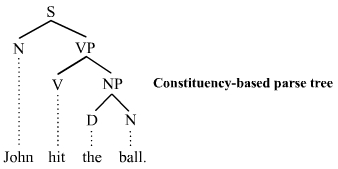
\includegraphics{figures/2_parsetree1}
  \caption[Syntactic Parse Tree Example]{Parse Tree for sentence "John hit the ball."\footnotemark \footnotetext{\url{https://upload.wikimedia.org/wikipedia/commons/5/54/Parse_tree_1.jpg}} }\label{fig:parsetree}
\end{figure}
\end{itemize} 

Once we have performed feature extraction, then the next step is to feed the feature input to the machine learning algorithm. There are a number of very successful and efficient supervised machine learning methods. They are described briefly as follows:
\begin{itemize}
\item \textbf{Na\"{i}ve Bayes:} A simple probabilistic classifier based on applying the Bayes' theorem with strong (naive) independence assumption.
\item \textbf{Maximum Entropy (ME):}  A probabilistic model that estimates the conditional distribution of the class label
\item \textbf{Support Vector Machines (SVM)} [Pang et al, \parencite{ch1:pang}] A representation of the examples as points in space in which support vectors are computed to provide a best division of points/examples into categories
\item \textbf{Logistic Regression (LR) Model} [Pang \& Lee,\parencite{ch2:panglee}] A LR model predicts the classes from a set of variables that may be continuous, discrete, or a mixture.
\end{itemize}

Since, the topics of this work are focused on exploring unsupervised word representations learned via deep learning and its application to the problem of sentiment analysis, we will not expand this discussion further.

\subsection{Domain Dependency Problem and Domain Adaptation}
When sentiment analysis is performed in real life, a common issue arises. A classifier trained using opinionated documents from domain A often performs poorly when tested on documents from domain B. There are genuine reasons for the same:
\begin{enumerate}
\item Reason 1: words used in different domains can be substantially different, e.g.
\begin{itemize}
\item Cars vs. Movies
\item Cameras vs. Strollers
\end{itemize}
\item Reason 2: some words mean opposite in two domains, e.g.
\begin{itemize}
\item “unpredictable” may be negative in a car review, but positive in a movie review [Turney, ACL 2002]
\item “cheap” may be positive in a travel/lodging review, but negative in a toys review
\end{itemize}
\end{enumerate}

A common way to mitigate this issue is \textbf{Domain Adaptation}. It's actually a well studied problem. [Aue \& Gamon~\parencite{ch2:auegamon}; Blitzer et al,~\parencite{BlitzerPaper:2007}; Yang et al,\parencite{ch2:yang}]. Some of the basic steps involved when perfroming domain adaptation is as follows:
\begin{enumerate}
\item Use labeled data from one domain and unlabeled data from both source the target domain and general opinion words as features
\item Choose a set of pivot features which occur frequently in both domains
\item Model correlations between the pivot features and all other features by training linear pivot predictors to predict occurrences of each pivot in the unlabeled data from both domains
\end{enumerate}
Recently, Jochim and Sch{\"u}tze \parencite{ch2:jochim} showed improvement in citation polarity classification using product reviews, by making use of Domain Adaptation, their out-of domain data was Amazon's Product Review data-set.

\section{Sentence-Level Sentiment Analysis}
Document level sentiment analysis is too coarse for most applications,\Smiley{} or, \Frowny{}? Example:
\newline

“I bought a new X phone yesterday. The voice quality is \textbf{super} and I really \textbf{like} it. However, it is a little bit \textbf{heavy}. Plus, the key pad is \textbf{too soft} and it \textbf{doesn’t feel comfortable}. I think the image quality is \textbf{good} enough but I am \textbf{not} sure about the battery life...”
\begin{itemize}
\item \textbf{Task:} Determine whether a sentence \textbf{s} is subjective or objective, and if \textbf{s} is subjective, determine whether its orientation is positive or negative
\item \textbf{Assumptions:} The sentence is opinionated on a single object and the opinion is from a single opinion holder.
\end{itemize}

It is important to highlight that at sentence level, the syntax becomes of paramount importance. Hence we begin next with understanding syntactic patterns.

\subsection{Syntactic Pattern Learning}
In thier 2003 work, Riloff and Wiebe~\parencite{ch2:reiloff} presented a bootstrapping process that learns linguistically rich extraction patterns for subjective (opinionated) expressions. The proposed process can be explained briefly as follows: 
\begin{enumerate}
\item Use high precision but low recall classifiers to automatically identify some subjective and objective sentences.
\begin{itemize}
\item A subjective classifier: the sentence contains two or more strong subjective clues
\item An objective classifier: the sentence contains no strong subjective clues
\item Based on manually collected single words and n-grams, which are good subjective clues
\end{itemize}
\item Learn a set of patterns from subjective and objective sentences identified above
\begin{itemize}
\item Syntactic templates are used to restrict the kinds of patterns to be discovered, e.g. <subject> active-verb $\Rightarrow$ the customer complained
\end{itemize}
\item The learned patterns are used to extract more subjective and objective sentences (the process can be repeated)
\end{enumerate}  

\section{Attribute - Level Sentiment Analysis}
We have seen from some of the reviews example presented earlier that a positive or a negative labeled document doesn't imply that the author likes or dislikes all attributes of the product. Thus, an interesting area of study is to analyze what attribute is most positively rated and which one is most negatively rated in a given product review. Also, in a general opinion corpus about a product, another interesting study is the percentage of positive to negative review for a given attribute. This is useful to determine, what exactly about the product do the people love or hate about the product. These attribute can be anything from product properties, the individual components or important topics etc. 

\begin{figure}[htb]
  \centering
  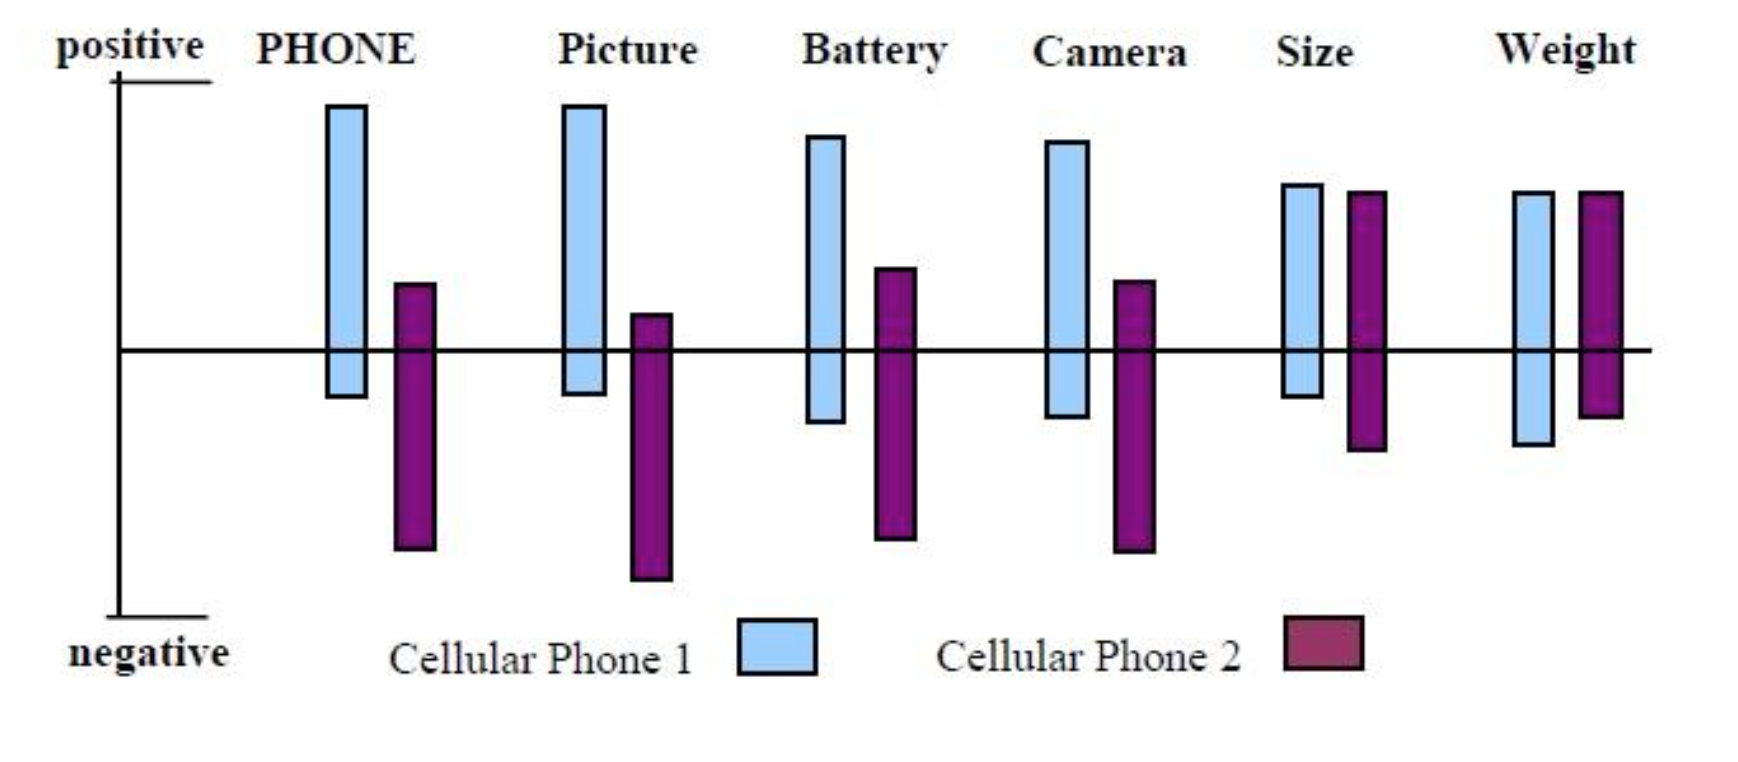
\includegraphics[width=130mm]{figures/2_attributesa}
  \caption[Sentiment Analysis - Attribute Level Example]{Attribute Level Sentiment Analysis Example }\label{fig:attributesa}
\end{figure}

The ~\autoref{fig:attributesa} shows an example of attribute level sentiment analysis. It displays the comparative analysis of two cellular phone and their individual attributes like positive or negative. Referring to the figure, one can clearly see that Cellphone 1 has overall positive sentiment, and it scores more positively for the attributes: picture, battery and camera. Where as, the size and weight of both the devices has received roughly similar reviews.

Again, there are many methods proposed which allows us to extract these attributes automatically. for the sake of focusing on this work, we will curtail the discussion here.  